\section{Kiến trúc hệ thống}
\indent Hệ thống được xây dựng theo mô hình MVC kết hợp với REST API (RESTful):
\subsection{Giới thiệu REST API:}
REST (REpresentational State Transfer) là một tiêu chuẩn thiết kế API (API architectural style) cho các ứng dụng. REST được giới thiệu lần đầu tiên bởi Roy Fielding vào năm 2000 trong luận án nổi tiếng của ông ``Architectural Styles and
the Design of Network-based Software Architecture'' đại học California.

Mặc dù REST có thể sử dụng trên hầu hết mọi giao thức ứng dụng phần mềm, nhưng REST thường biết đến rộng rãi trong các giao thức của ứng dụng Web vì tận dụng được những lợi thế của HTTP, giúp nhà phát triển không cần cài đặt thêm phần mềm hoặc thư viện bổ sung để sử dụng REST API.

Một số đặc điểm cơ bản của REST:
\begin{itemize}
    \item \textbf{Uniform interface:} Các API được thiết kế một cách nhất quán theo các nguyên tắc chung. Ví dụ luôn luôn sử dụng danh từ số nhiều thay vì khi số nhiều, khi số ít, sử dụng dấu gạch ngang để phân tách giữa các từ. Tài nguyên của hệ thống phải tuân theo các quy tắt đặt tên, định dạng dữ liệu (JSON hay XML), được truy cập thông qua một cách tiếp cận phổ biến như HTTP GET và được sửa đổi thông qua các phương thức tương tự.
    \item \textbf{Client-Server:} Client và Server không cần phụ thuộc vào nhau, có thể phát triển độc lập, thậm chí sửa đổi, thay thế miễn sao interface giao tiếp giữa chúng vẫn được giữ nguyên.
    \item \textbf{Stateless (Không trạng thái)}: Server không lưu trữ bất kì thông tin gì về yêu cầu của client, nó sẽ coi mọi yêu cầu là mới. Không section, không history. Vì vậy, mỗi yêu cầu từ client tới server phải chứa tất cả các thông tin cần thiết để  server hiểu được yêu cầu đó.
    \item \textbf{Code on demand:} Sử dụng HTTP status code khi có thể
\end{itemize}


Những lợi ích khi sử dụng REST API:

- Nhờ tính độc lập giữa client và server, ta có thể dễ dàng sửa đổi, thay thế mà không lo lắng nhiều vấn đề.

- API REST luôn độc lập với loại nền tảng hoặc ngôn ngữ: API REST luôn thích nghi với loại cú pháp hoặc nền tảng đang được sử dụng, điều này mang lại sự tự do đáng kể khi thay đổi hoặc kiểm tra môi trường mới trong quá trình phát triển. Với API REST, bạn có thể có máy chủ PHP, Java, Python hoặc Node.js. Điều duy nhất là không thể thiếu rằng các phản hồi cho các yêu cầu phải luôn diễn ra bằng ngôn ngữ được sử dụng để trao đổi thông tin, thông thường là XML hoặc JSON.

Vận dụng kiến trúc REST API trong hệ thống:
Các API trong hệ thống được thiết kế theo các nguyên tắc chung, nhất quán giữa các module.
\begin{itemize}
    \item API được đặt tên theo quy định chung, phù hợp với tác dụng của API, thống nhất giữa các module. %Them vi du
    \item Sử dụng các phương thức HTTP (GET, POST, PUT, DELETE) để truy cập và xử lý dữ liệu. %Them vi du
    \item Dữ liệu được trả về theo định dạng JSON. %Them vi du
    \item Server trả về các HTTP code phù hợp. %Them vi du
\end{itemize}
\section{Mô hình Model-View-Controller:}
Nhận thấy mô hình MVC có nhiều ưu điểm và phù hợp với hệ thống (trình bày ở mục 2.1 Mô hình Model-View-Controller) nên nhóm đã sử dụng MVC trong thiết kế kiến trúc hệ thống.

Vận dụng mô hình MVC trong hệ thống:
\begin{center}
  \captionsetup{type=figure}
  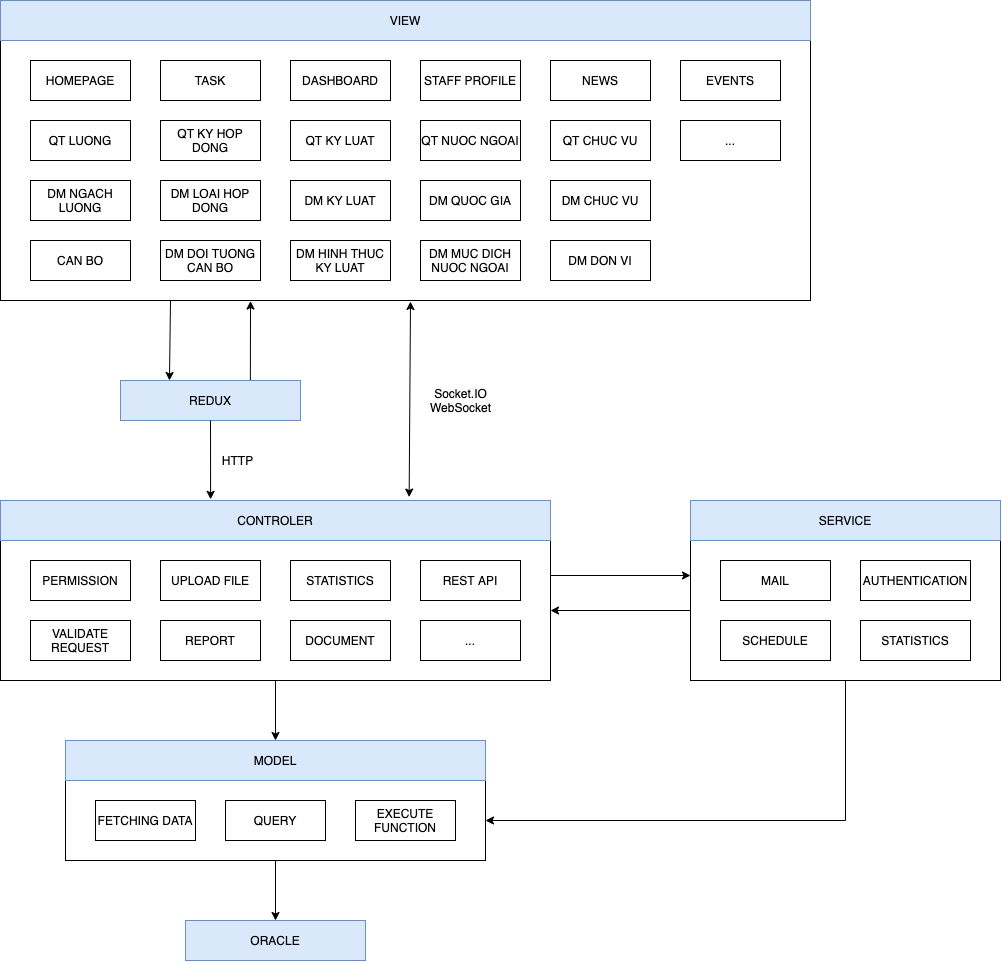
\includegraphics[width=15cm]{img/MVCInTchc.png}
  \captionof{figure}{Mô hình MVC kết hơp với Redux trong hệ thống}
\end{center}

\section{Nguyên tắc thiết kế hệ thống}
\indent Với một hệ thống khá phức tạp như trên cần phải có những nguyên tắc thiết kế chung
\subsection{Cấu trúc cây thư mục của mã nguồn}
\indent Việc cần làm đầu tiên và quan trọng nhất là tổ chức files và các thư mục. Với một thiết kế tốt thì khi làm việc chung giữa nhiều người sẽ ít bị đụng độ. Nhóm lựa chọn cách chia mỗi thành phần của trang ra từng module tách biệt với nhau, thuận lợi cho việc mở rộng và bảo trì, bảo dưỡng. Bên dưới là cấu trúc mã nguồn mà nhóm đã lựa chọn:
\begin{center}
  \captionsetup{type=figure}
  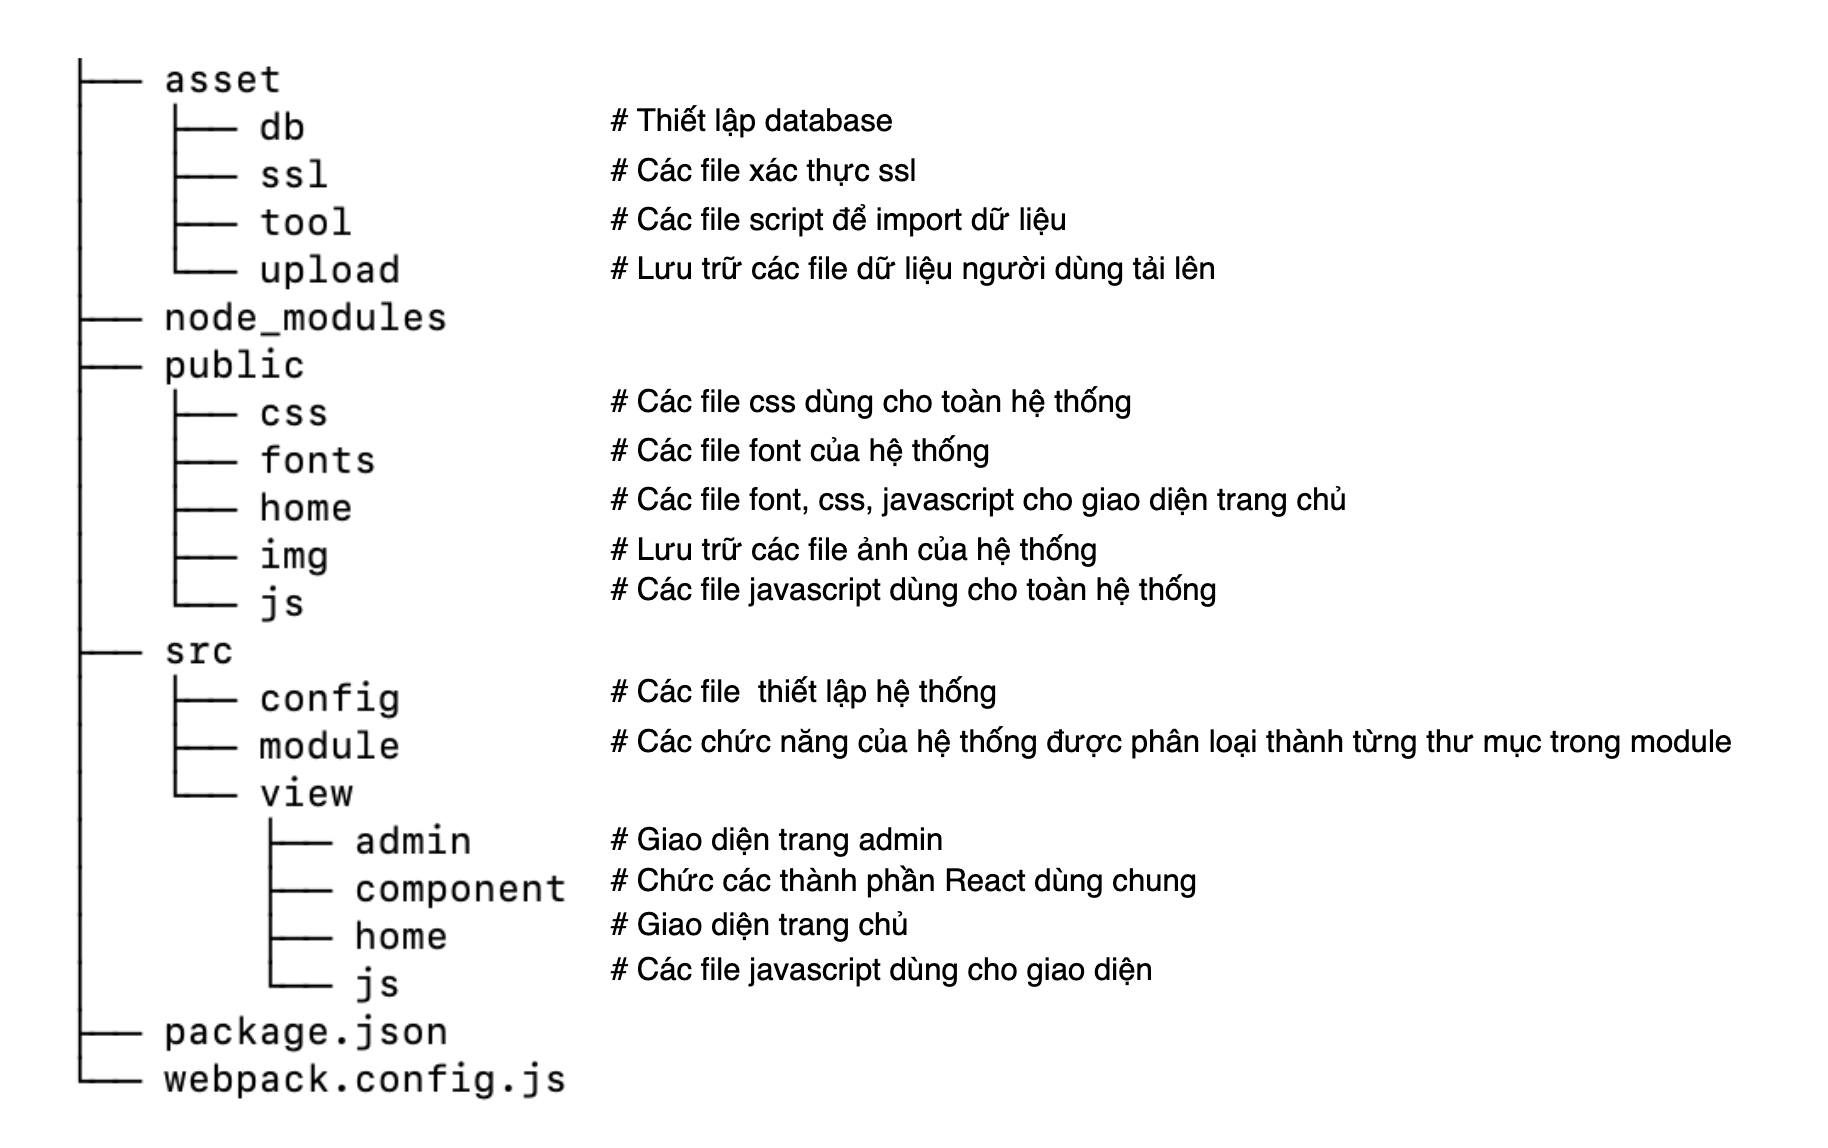
\includegraphics[width=15cm]{img/tree.png}
  \captionof{figure}{Cây thư mục của hệ thống}
\end{center}
\section{Thiết kế đối tượng người dùng}
\subsection{Danh sách đối tượng người dùng}
\begin{table}[H]
    \centering
	\begin{tabular}{|p{1cm}|p{4cm}|p{10cm}|}
    \hline
    \textbf{STT}&\textbf{Người dùng}&\textbf{Đặc tả}\\
	\hline
    1&Quản trị hệ thống&Là những người tạo ra hệ thống ban đầu, có các chức năng hỗ trợ tạo ra các cấu hình cho hệ thống, bao gồm các thao tác như: cấu hình các thông tin chung của phòng Tổ chức hành chính, cấu hình về giao diện, quản lý tài khoản người dùng\\
	\hline
    2&Trưởng phòng Tổ chức - Hành chính&Chức năng chính là chịu trách nhiệm phân công công việc cho các cán bộ thuộc phòng Tổ chức - Hành chính. Bên cạnh đó những người này còn có chức năng quản lý thông tin của cán bộ nhà trường\\
	\hline
    3&Cán bộ phòng Tổ chức - Hành chính&Là những cán bộ thuộc phòng Tổ chức - Hành chính. Họ có chức năng quản lý thông tin của toàn bộ cán bộ, quản lý thông tin các danh mục , quản lý thông tin các quá trình nghiệp vụ của nhà trường.\\
	\hline
	4&Người dùng (giảng viên, cán bộ nhà trường)&Người dùng với mục đích quản lý được thông tin, các quá trình nghiệp vụ của bản thân.\\
	\hline
\end{tabular}
\caption{Danh sách đối tượng người dùng của hệ thống}
\end{table}
\subsection{Đối tượng: Quản trị hệ thống}
\textbf{Lược đồ Usecase tổng thể}
\begin{center}
  \captionsetup{type=figure}
  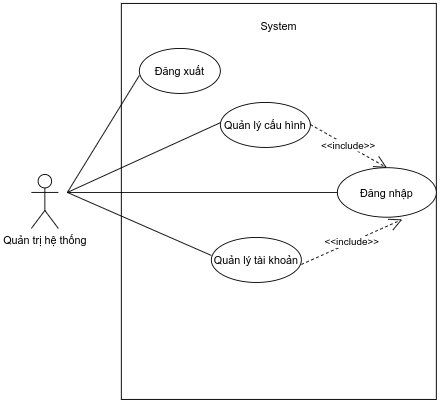
\includegraphics[scale=0.8]{img/UML/Admin/adminUsecase.png}
  \captionof{figure}{Lược đồ usecase của đối tượng quản trị hệ thống}
\end{center}

\indent Đối với đối tượng là quản trị hệ thống, sau khi xác thực thành công sẽ cónhững nhóm chức năng: quản lý tài khoản và quản lý cấu hình.Với mỗi nhóm chức năng sẽ có những chức năng tương ứng được thể hiện trong các lược đồ Usecase sau:

\begin{center}
  \captionsetup{type=figure}
  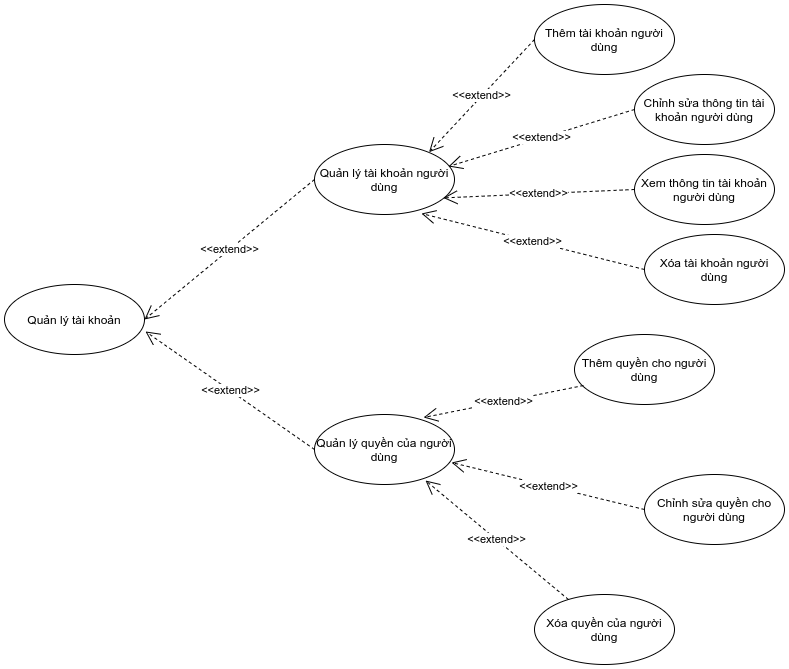
\includegraphics[scale=0.5]{img/UML/Admin/quanlytaikhoan.png}
  \captionof{figure}{Lược đồ Usecase cho nhóm chức năng quản lý tài khoản}
\end{center}

Trong nhóm quản lý tài khoản bao gồm các chức năng: quản lý tài khoản người dùng và quản lý quyền của người dùng.
\begin{itemize}
    \item Quản lý tài khoản người dùng:
        \subitem Người quản trị có thể thay các tài khoản với các quyền đặc biệt cho trưởng phòng Tổ chức - Hành chính, cán bộ phòng Tổ chức - Hành chính
    \item Quản lý quyền của người dùng:
        \subitem Người quản trị hệ thống có thể thêm một quyền mới vào hệ thống, chỉnh sửa quyền, xóa quyền, cũng như gắn quyền cho người dùng nhất định.
\end{itemize}

\begin{center}
  \captionsetup{type=figure}
  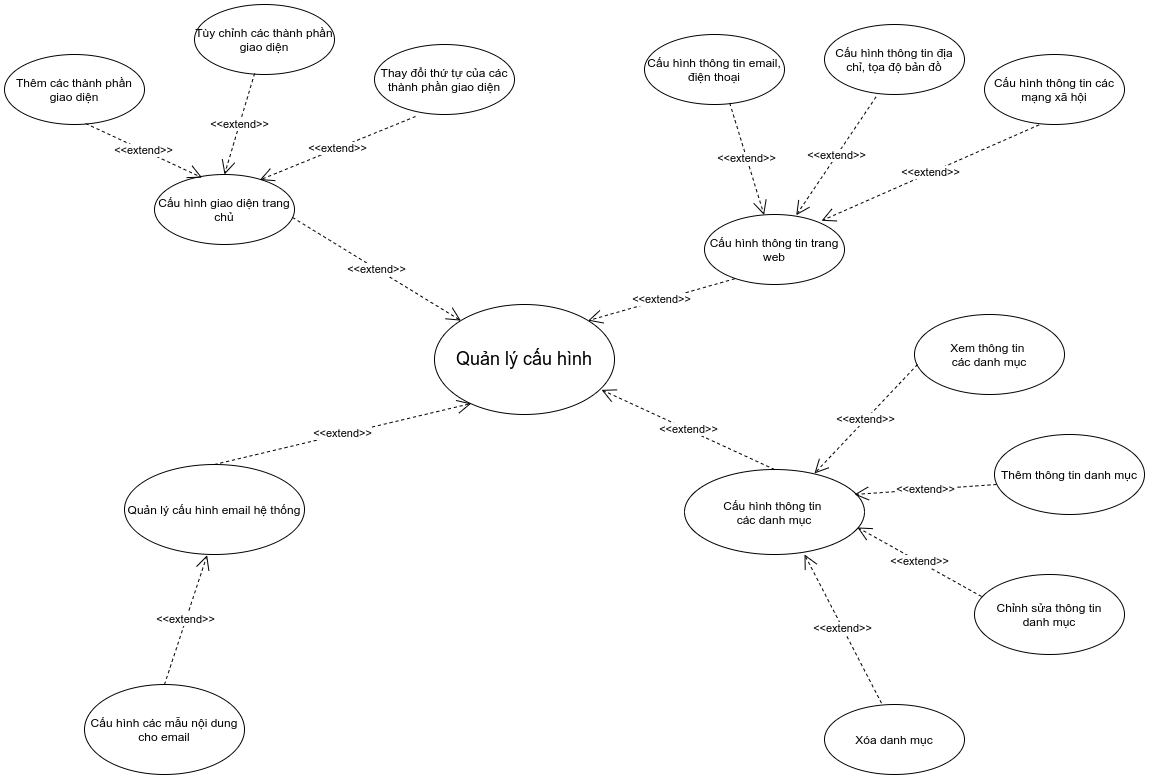
\includegraphics[scale=0.4]{img/UML/Admin/quanlycauhinh.png}
  \captionof{figure}{Lược đồ Usecase cho nhóm chức năng quản lý cấu hình}
\end{center}

Nhóm quản lý cấu hình gồm các chức năng: cấu hình giao diện trang chủ, cấu hình thông tin trang web, cấu hình email cho hệ thống, cấu hình thông tin danh mục.

- Cấu hình giao diện trang chủ: Tùy chỉnh các thành phần giao diện, lựa chọn các thành phần giao diện sẽ xuất hiện ở trang chủ.

- Cấu hình thông tin trang web: Cấu hình các thông tin chung cho hệ thống, thông tin liên lạc của phòng Tổ chức - Hành chính.

- Cấu hình email hệ thống: Tủy chỉnh các mẫu email tự động của hệ thống.

- Cấu hình thông tin các danh mục: Xây dựng thông tin những danh mục mặc định phục vụ cho việc nhập và lữu trữ dữ liệu trong hệ thống.
\subsection{Đối tượng: Trường phòng Tổ chức - Hành chính}
\textbf{Lược đồ Usecase tổng thể}
\begin{center}
  \captionsetup{type=figure}
  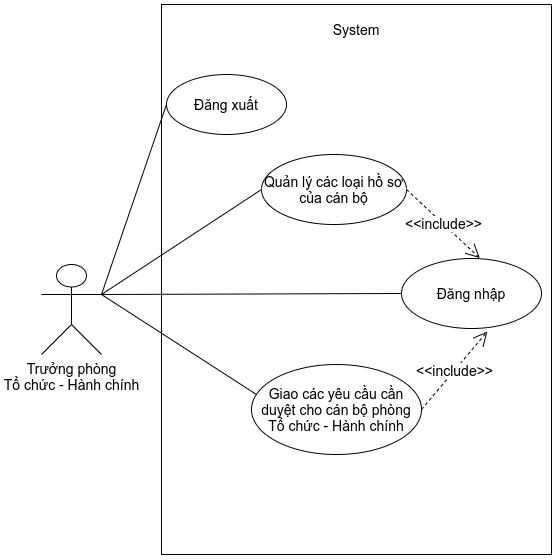
\includegraphics[scale=0.7]{img/UML/Manager/truongphong.png}
  \captionof{figure}{Lược đồ Usecase cho đối tượng Trường phòng Tổ chức - Hành chính }
\end{center}
Đối với đối tượng là Trưởng phòng Tổ chức - Hành chính sau khi đăng nhập sẽ có những nhóm chức năng sau: quản lý thông tin các loại hồ sơ của từng cán bộ, giao các yêu cầu cần duyệt cho cán bộ thuộc phòng Tổ chức - Hành chính